
\bpar{
\chapter*{General opening}
}{
\chapter*{Ouvertures Générales}
}

\bpar{
\markboth{General opening}{General opening}
}{
\markboth{Ouvertures générales}{Ouvertures générales}
}

\label{ch:opening}

%----------------------------------------------------------------------------------------

%\newpage


\bpar{
As we suggested before, the opening in fact allows to take a step back and in our case a clarification of the global frame. We therefore propose here the exercise to summarize already invoked opening works, questions opened by our work, and their synthesis within a long term research project.
}{
Comme nous l'avons suggéré précédemment, l'ouverture permet en fait une prise de recul et dans notre cas une clarification du cadre global. Nous proposons donc ici l'exercice de recension des travaux d'ouverture déjà menés, celle des problèmes ouverts par notre travail, et leur synthèse dans un projet de recherche à long terme.
}


%%%%%%%%%%
\section*{Thematic and general perspectives}{Perspectives thématiques et générales}



%%%%%%%%%%
\subsection*{Into a global perspective}{Mise en perspective globale}



\bpar{
A second reading of the thesis enlightened by the theoretical articulation proposed in~\ref{sec:theory} confirms us that (i) the morphogenetic approach was naturally induced by the constraint of ecological niche in the definition of co-evolution; (ii) the evolutive urban theory is thus refined for the precise cas of co-evolution; (iii) territorial systems must intrinsically induce such processes, since they are both support and objects of these. The question of network necessity to represent territorial systems remains open, and we have postulated it in our theoretical construction. Our results suggest the relevance to take them into account, and open the question of a demonstration of this postulate.
}{
Une relecture de la thèse à la lumière de l'articulation théorique proposée en~\ref{sec:theory} nous confirme que (i) l'approche morphogénétique était naturellement induite par la contrainte de niche écologique dans la définition de la co-évolution ; (ii) la théorie évolutive des villes est ainsi précisée pour le cas précis de la co-évolution ; (iii) les systèmes territoriaux doivent intrinsèquement induire de tels processus, puisqu'ils sont à la fois support et objets de ceux-ci. La question de la nécessité des réseaux pour représenter les systèmes territoriaux reste ouverte, et nous l'avons postulée dans notre construction théorique. Nos résultats suggèrent la pertinence de leur prise en compte, et ouvrent la question d'une démonstration de ce postulat.
}


\bpar{
Then, a third reading through knowledge domains allows to better understand the articulation between the different components: conceptual and empirical constructions of the first part yield a definition of co-evolution, and the elaboration of methods and models in a second part, which in turn feed back these other domains in the third part. We propose a brief quantitative analysis of these dynamics in~\ref{app:reflexivity}. Therefore, the interdependancy within the path taken, given by the diagram in introduction (Frame~\ref{frame:intro:organisation}), is indeed much more complex and not necessarily linear. Renewed readings of this monograph will thus be richer, through the emergence of implicit links. We propose in Frame~\ref{frame:opening:organisation} a possible new reading of the organisation of our work, in relation to the general problematic and knowledge domains. 
}{
Ensuite, une relecture par les domaines de connaissance permet de mieux comprendre l'articulation entre les différentes composantes : les constructions conceptuelles et empiriques de la première partie permettent une définition de la co-évolution, puis la mise en place de méthodes et de modèles en deuxième partie, qui en retour alimentent ces autres domaines en troisième partie. Nous proposons une analyse quantitative brève de ces dynamiques en~\ref{app:reflexivity}. Ainsi, l'interdépendance dans le cheminement, donnée par le diagramme en introduction (Encadré~\ref{frame:intro:organisation}), est en fait bien plus complexe et pas forcément linéaire. Une deuxième lecture de notre monographie sera ainsi plus riche, par émergence des liens implicites. Nous proposons en Encadré~\ref{frame:opening:organisation} une relecture possible de l'organisation de notre travail, au regard de la problématique générale et des domaines de connaissance.
}



%%%%%%%%%%%%%%
\begin{figure}
	\begin{mdframed}
	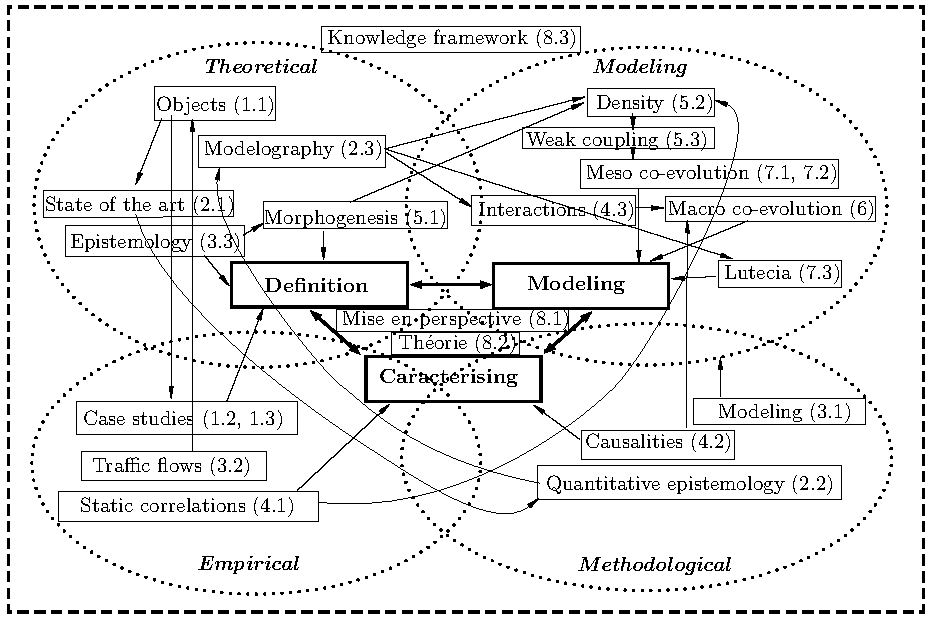
\includegraphics[width=\linewidth]{Figures/Theory/orga.pdf}
	\medskip
	\framecaption{\textbf{Rereading of the organisation at the light of knowledge domains.} We put at the core the three axis coming from the general problematic, of defining, characterizing and modeling co-evolution. Different components irrigate its elements which can not be dissociated, and finally blended together by the conclusion and opening. Sections are located in an indicative way within the knowledge domain which corresponds the most (knowing that they are all across different domains). The domains of data and tools are here let aside to facilitate reading (and would necessitate a more precise description of the work). The relations between components are also given in an indicative way and are not exhaustive, but allow to grasp the complexity of the global articulation.\label{frame:opening:organisation}}{\textbf{Relecture de l'organisation à la lumière des domaines de connaissance.} Nous plaçons au coeur le triptyque issu de la problématique générale de définition, caractérisation et modélisation de la co-évolution. Différentes composantes irriguent ses éléments qui sont indissociables, et soudés finalement par la conclusion et ouverture. Les sections sont placées à titre indicatif dans le domaine de connaissance qui leur correspond le plus (sachant qu'elles sont toutes à cheval sur plusieurs domaines). Les domaines de données et outils sont laissés de côté ici pour faciliter la lecture (et nécessiteraient un découpage plus précis du travail). Les relations entre composantes sont également données à titre indicatif et ne sont pas exhaustives, mais permettent de se rendre compte de la complexité de l'articulation globale.\label{frame:opening:organisation}}
	\end{mdframed}
\end{figure}
%%%%%%%%%%%%%%



\bpar{
Our work can also be inserted within a broader perspective. Let precise the ``meta-articulation'' of our work, i.e. the implicit structure of the diverse developments and openings and therefore the global frame in which the core is integrated (first three parts). The Frame~\ref{frame:opening:perspective} gives a schematic representation of this articulation. The core, which consists in the answer to the problematic, is constituted by three axis in strong interaction: the definition, the characterization and the modeling of co-evolution of transportation networks and territories. Each call in its way to developments in different fields\footnote{We do not use the term of domain here to avoid a confusion with knowledge domains, these being used in a different way as we will see in Appendix~\ref{app:reflexivity}.}: contributions in epistemology and quantitative epistemology, mainly linked to the aspect of definition; development of systemic frameworks, induced by issues linked to modeling; and thematic developments linked to the characterization.
}{
Notre travail peut également se placer dans une perspective plus large. Précisons la ``méta-articulation'' de notre travail, c'est-à-dire la structure implicite des divers développements et ouvertures et donc le cadre global dans lequel s'inscrit le coeur (trois premières parties). L'Encadré~\ref{frame:opening:perspective} schématise cette articulation. Le coeur, qui consiste en la réponse à la problématique, est constitué de trois axes en interaction forte : la définition, la caractérisation et la modélisation de la co-évolution des réseaux de transport et des territoires. Chacun appelle à sa manière des développements dans divers champs\footnote{Nous n'utilisons pas le terme domaine ici pour ne pas entrainer une confusion avec les domaines de connaissance, ceux-ci étant mobilisés différemment comme nous le verrons en Annexe~\ref{app:reflexivity}.} : des développements épistémologiques et en épistémologie quantitative, principalement liés à l'aspect de définition ; des développements de cadres systémiques, induits par les problématiques liées à la modélisation ; et des développements thématiques liés à la caractérisation.
}


\bpar{
We can detail the content of each of these developments, by linking them to the corresponding content mainly in Appendices:
\begin{enumerate}
	\item Quantitative epistemology: mostly in relation with methods and tools for systematic review and exploration of a scientific landscape in~\ref{ch:modelinginteractions}, we include the original case study which initiated the method, the corpus of the Cybergeo journal, in~\ref{app:sec:cybergeo}, and also an application to a massice patent corpus in~\ref{app:sec:patentsmining}.
	\item Epistemology: contextualizing the study of Cybergeo with other complementary approaches yields epistemological considerations in~\ref{app:sec:cybergeonetworks}; we also start a reflexion on the links between economics and geography in~\ref{app:sec:ecogeo}.
	\item Systemic frameworks: a knowledge framework, contributing to organize a complex knowledge, has already been proposed in~\ref{sec:knowledgeframework}; a framework formalizing the coupling of models of socio-technical systems, suggesting directions to formalize the knowledge framework, is developed in~\ref{app:sec:csframework}; a framework to study the robustness of multi-attribute evaluations is developed in~\ref{app:sec:robustness}.
	\item Thematical: the case studies of transportation systems achieved in \ref{sec:reproducibility} and in~\ref{sec:energyprice} provide indeed a confirmation of relevant scales; the study of the generation of synthetic data, in relation with the methodology developed in~\ref{sec:computation}, is done in~\ref{app:sec:syntheticdata} for the method and in~\ref{app:sec:syntheticdata-finance} for an example of application; the modeling of migration dynamics within Pearl River Delta sketched in~\ref{app:sec:migrationdynamics}, introduces elements for multi-scale models and refines interactions between cities at the level of individual flows.
\end{enumerate}
}{
Détaillons le contenu de chacun de ces développements, en les reliant au contenu correspondant principalement en Annexes :
\begin{enumerate}
	\item Epistémologie quantitative : principalement en lien avec les méthodes et outils de revue systématique et d'exploration d'un paysage scientifique en~\ref{ch:modelinginteractions}, nous incluons le cas d'étude original qui a initié la méthode, le corpus du journal Cybergeo, en~\ref{app:sec:cybergeo}, ainsi qu'une application à un corpus massif de brevets en~\ref{app:sec:patentsmining}.
	\item Epistémologie : la mise en contexte de l'étude de Cybergeo avec d'autres approches complémentaires permet une prise de recul épistémologique dans~\ref{app:sec:cybergeonetworks} ; nous amorçons également une réflexion sur les liens entre économie et géographie en~\ref{app:sec:ecogeo}.
	\item Cadres systémiques : un cadre de connaissance, contribuant à organiser une connaissance complexe, a déjà été proposé en~\ref{sec:knowledgeframework} ; un cadre formalisant le couplage des modèles des systèmes socio-techniques, suggérant des pistes de formalisation du cadre de connaissance, est développé dans~\ref{app:sec:csframework} ; un cadre pour l'étude de la robustesse des évaluations multi-attributs est développé dans~\ref{app:sec:robustness}.
	\item Thématique : les études de cas des systèmes de transport effectuées en \ref{sec:reproducibility} et en~\ref{sec:energyprice} permettent en l'occurence une confirmation des échelles pertinentes ; l'étude de la génération de données synthétiques, en lien avec la méthodologie développée en~\ref{sec:computation}, est faite en~\ref{app:sec:syntheticdata} pour la méthode et en~\ref{app:sec:syntheticdata-finance} pour un exemple d'application ; la modélisation des dynamiques migratoires au sein du Delta de la Rivière des Perles ébauchée en~\ref{app:sec:migrationdynamics}, introduit une piste de modèles multi-échelle et raffine les interactions entre villes au niveau des flux individuels.
\end{enumerate}
}


%%%%%%%%%%%%%%
\begin{figure}
	\begin{mdframed}
	\bpar{
	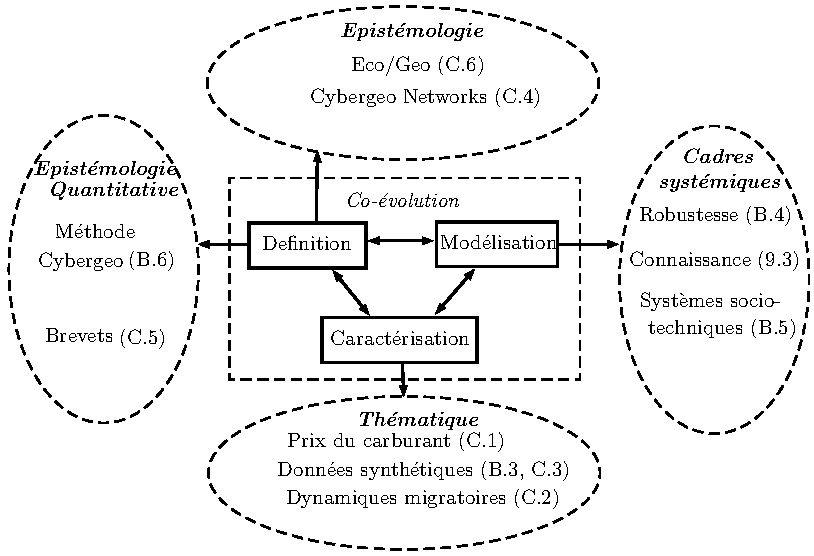
\includegraphics[width=\linewidth]{Figures/Theory/metacadre_norefs.pdf}
	}{
	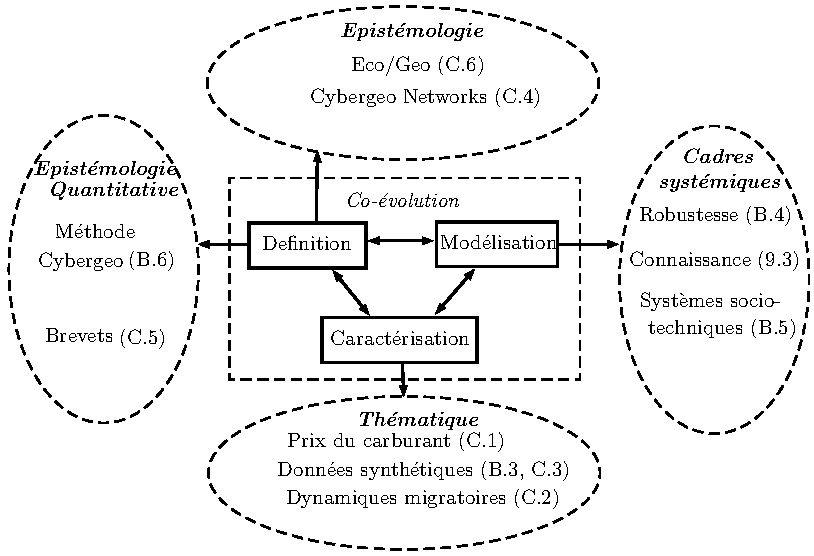
\includegraphics[width=\linewidth]{Figures/Theory/metacadre_norefs_fr.pdf}
	}
	\medskip
	\framecaption{\textbf{Perspective on the global frame.} The core of the problematic, co-evolution, is composed by three components which call for extensions within diverse fields (their intersections being not represented to ease reading). We list here within each the different openings, mainly done in Appendices.\label{frame:opening:perspective}}{\textbf{Mise en perspective du cadre global.} Le coeur de la problématique, la co-évolution, est composé de trois composantes qui appellent des extensions dans des champs divers (leurs intersections n'étant pas représentées pour faciliter la lecture). Nous y listons dans chaque les différentes ouvertures, menées principalement en Annexes.\label{frame:opening:perspective}}
	\end{mdframed}
\end{figure}
%%%%%%%%%%%%%%



\bpar{
These different fields have naturally non-empty intersections (the knowledge framework of~\ref{sec:knowledgeframework} corresponds for example both to a systemic framework and to epistemology, or the study of patents is an important thematic aspect in link with the evolutive urban theory) and are interacting: studies in quantitative epistemology inform epistemology, what guides thematic studies, which can be put into perspective in the systemic frameworks, which in their turn also depend on the epistemological positioning.
}{
Ces différents champs sont bien sûr à intersections non vides (le cadre de connaissance de~\ref{sec:knowledgeframework} relève par exemple à la fois du cadre systémique et de l'épistémologie, ou l'étude des brevets est un important aspect thématique en lien avec la théorie évolutive des villes) et en interactions : les études d'épistémologie quantitative informent l'épistémologie, qui guide les études thématiques, qui peuvent être mises en perspective dans les cadres systémiques, qui eux dépendent également du positionnement épistémologique.
}


\bpar{
Thus, we highlight a more global structure for our work, which partly sketches the structure of a research project that we will detail in the following.
}{
Ainsi, nous mettons en évidence une structure plus globale pour notre travail, qui dessine en partie la structure d'un projet de recherche que nous détaillerons par la suite.
}



% \paragraph{External integration}
%At all stages of my thesis project, different types of reflexivity play a crucial role and allow to enlarge the scope of results and theories constructed. I also led some auxiliary projects with aim to increase the integration of my work within disciplines and knowledge domains. For example, in the domain of methodology, \cite{raimbault2017discrepancy} investigates the quantification of robustness of multi-attribute optimisations, that can apply to any type of complex systems. Scientific communication is also a crucial aspect for socio-technical systems, and \cite{raimbault2016game} is an exploration of using agent-based modeling to transmit concepts in ecology. The work of \cite{raimbault2016indirect} was done in the frame of the collaborative development of an interactive platform to explore scientific corpuses, with the aim to promote open science and reflexivity. % These two examples are in the domain of tools, which both can apply to our work and link it to broader fields. 
%Finally, I also explored empirical questions close to my research subjects, such as technological innovation. The diffusion of innovations between cities is indeed one crucial components of the Evolutive Urban Theory. In \cite{bergeaud2017classifying}, we extended the corpus analysis tools to apply to the full corpus of US Patents spanning 1976-2012, to create an endogenous classification that we show to be complementary to the existing office classification. This opens ways for future projects, as the combination with existing inventor localisation databases is a potential candidate for empirical testing of the diffusion hypothesis of the Evolutive Urban Theory. Such a knowledge loop is an illustration how integration of fields can be beneficial. 






\subsection*{Open questions}{Questions ouvertes}


\bpar{
We now develop fundamental questions which have been evoked or opened all along our work, which we classify into three axis: scientific practice (applied epistemology), modeling, and foundations of spatial complex systems.
}{
Nous développons à présent des questions fondamentales qui ont été abordées ou ouvertes tout au long de notre travail, que nous classons en trois axes : pratique scientifique (épistémologie appliquée), modélisation, et fondements des systèmes complexes spatiaux.
}


\subsubsection*{Applied epistemology}{Epistémologie appliquée}


\paragraph{For a completely open science}{Pour une science totalement ouverte}

\bpar{
A first crucial axis of development for all the ecosystem of knowledge production within which we are integrated (see chapter~\ref{ch:positioning}) is the contribution to a maximal opening of the scientific practice, i.e. the combination of all the approaches summarized by \cite{fecher2014open}, in particular the democratic and public aspects which foster the access of all to the production of knowledge and its results\footnote{Knowing that the opening of knowledge products is intrinsic in a complex perspective, since as \cite{morin1991methode} puts it, our ideas find a certain independence in the noosphere and do not belong to us.}, and the pragmatic and infrastructure aspects which focuses on the increased efficiency within an open framework.
}{
Un premier axe de développement crucial pour l'ensemble de l'écosystème de production de connaissance dans lequel nous nous inscrivons (voir chapitre~\ref{ch:positioning}) est la contribution à une ouverture maximale de la pratique scientifique, c'est-à-dire la combinaison de l'ensemble des approches résumées par \cite{fecher2014open}, en particulier les aspects démocratique et public qui encouragent l'accès de tous à la production de connaissance et à ses résultats\footnote{Sachant que l'ouverture des produits de la connaissance est évidente dans une perspective complexe, puisque comme le souligne \cite{morin1991methode}, nos idées prennent une certaine indépendance dans la noosphère et ne nous appartiennent pas.}, et les aspects pragmatique et d'infrastructure qui appuient l'efficience augmentée dans un cadre ouvert.
}


\bpar{
Transparency and availability of raw data or at least preprocessed data, and of the computer code producing simulation outputs or figures, seems to be more an exception than the rule in geography. As recalls \cite{banos2013pour} which consecrates one of its principles to it, ``\textit{the modeler is not the guardian of the proofed truth}'', and as recalled in~\ref{sec:reproducibility}, a perfect reproducibility of results is necessary for any value to be acknowledged by the scientific community, as a theory which does not provide falsification possibilities can not be considered as scientific in the sense of \noun{Popper}. Reviewing experiences for \emph{Cybergeo} have confirmed with unanimity this fundamental issue. We can recall that the journal \emph{PNAS} imposes to provide raw data and tables producing any figure, to prevent any visualization bias let it be voluntary (what is crippling and leads to a signalling) or not.
}{
La transparence et mise en disponibilité des données brutes ou au moins pré-traitées, et du code informatique produisant les sorties de simulation ou les figures, semble être plutôt l'exception que la règle en géographie. Comme le rappelle \cite{banos2013pour} qui y dédie l'un de ses principes, ``\textit{le modélisateur n'est pas le gardien de la vérité prouvée}'', et comme rappelé en~\ref{sec:reproducibility}, une reproductibilité parfaite des résultats est nécessaire pour une reconnaissance d'une quelconque valeur par la communauté scientifique, comme une théorie qui ne fournit pas de possibilité de falsification ne peut être considérée comme scientifique au sens de \noun{Popper}. Des experiences de revue pour \emph{Cybergeo} ont confirmé à l'unanimité ce problème fondamental. Rappelons que la revue \emph{PNAS} exige les données brutes et tableau produisant toute figure, pour prévenir tout biais de visualisation qu'il soit volontaire (ce qui est rédhibitoire et conduit à un signalement) ou non.
}


\bpar{
Furthermore, scientific communication is an important aspect of open science. The current mode of scientific publishing is far from being ideal. An article is not an understandable format nor really reproducible, and leads to bias. The writing of a paper while answering to the norms in order to be accepted can be assimilated to ``a game'' which rules are subtle and must be mastered to follow a carrier. According to our positioning, such a communication mode is contrary to the honesty and intellectual integrity which are necessary for an ethical and open science. Initiatives multiply to propose alternative models: post-publication review is one, the use of version control systems and public repositories is an other, or the flash publication of research directions\footnote{See for example the \emph{Journal of Brief Ideas} at \url{http://beta.briefideas.org/about}. Short descriptions of research directions are often delegated to the discussion of the conclusion of papers, which are written in a conventional way, often with a bias to justify a posteriori the interest of \emph{our new method} which unfortunately must be sold. We therefore build gigantic plans, propose developments with few connections, or application domains \emph{which will have an impact} (read which are fashionable or receive the most financing at the period of writing). This manuscript naturally falls under these critics, as do the associated papers.}. For example, \cite{bon2017novel} describes an experiment of dynamical articles evaluated in an open way by the community, with associated metrics allowing to make the works judged as interesting emerge.
}{
Par ailleurs, la communication scientifique est un aspect important de la science ouverte. Le mode actuel de publication scientifique est loin d'être idéal. Un article n'est pas un format compréhensible ni vraiment reproductible, et pousse au biais. L'écriture d'un article en répondant au normes de façon à être accepté peut être assimilé à ``un jeu'' dont les règles sont subtiles et qu'il faut maitriser pour faire carrière. Selon notre positionnement, un tel mode de communication est contraire à l'honnêteté et l'intégrité intellectuelle nécessaires à une science éthique et ouverte. Les initiatives se multiplient pour proposer des modèles alternatifs : la revue post-publication en est une, l'utilisation de systèmes de contrôle de version et de dépôts publics une autre, ou la publication éclair de pistes de recherche\footnote{Voir par exemple le \emph{Journal of Brief Ideas} à \url{http://beta.briefideas.org/about}. Les descriptions courtes de pistes de recherche sont souvent reléguées à la discussion ou la conclusion des articles, qui s'écrivent de manière conventionnelle, souvent avec un biais pour justifier a posteriori l'intérêt de \emph{sa nouvelle méthode} qu'il faut malheureusement vendre. On fait alors des plans sur la comète, propose des développements ayant peu de rapport, ou des domaines d'application \emph{qui auront un impact} (lire qui sont à la mode ou qui reçoivent le plus de financements à la période de l'écriture). Ce manuscrit tombe bien évidemment partiellement sous ces critiques, comme les articles qui lui sont associés.}. Par exemple, \cite{bon2017novel} décrit une expérience d'articles dynamiques évalués de manière ouverte par la communauté, avec des métriques associées permettant de faire émerger les travaux jugés intéressants.
}

% Journal of Design and Science ; Journal mec Paris Sud (CEA ?)


%%%%%
%% -- TRAD
%%%%%

\bpar{
Similarly, we claim that a linear presentation of a research project is too much reducing, and that the invention of alternative communication modes is a future issue for open science. We can for example imagine interactive networks, translating the structure of the underlying knowledge, and in which the reader can navigate between concepts and analyses, being 
}{
De la même façon, nous soutenons qu'une présentation linéaire d'un projet de recherche est trop fortement réducteur, et que l'invention de modes de communication alternatifs est un enjeu futur pour la science ouverte. On peut par exemple imaginer des réseaux interactifs, traduisant la structure de la connaissance sous-jacente, et dans lesquels le lecteur peut naviguer entre les concepts et les analyses, être renvoyé directement vers les données, modèles et analyses. Les grilles de lecture principales en accord avec l'argument que prendrait une explication linéaire peuvent alors être superposées au réseau pour revenir à un mode plus classique de lecture. Une communication par le jeu est également une alternative crédible, notamment dans le cas d'une communication pour le public, et nous en donnons une illustration pour un problème d'écologie en Annexe~\ref{app:sec:mediationecotox}.
}


\paragraph{For an evidence-based science}{Pour une science evidence-based}

Nous postulons qu'une science entièrement \emph{evidence-based}, quel que soit son objet, est possible et souhaitable en articulation avec la science ouverte. L'idée est de chercher à déconnecter la connaissance scientifique de tout dogmatisme, de tout a priori politique et de tout jugement de valeur\footnote{Sachant que par ailleurs ceux-ci doivent être plus que jamais développés et réfléchis pour articuler la science avec la société, mais doivent le moins possible interférer avec le processus de production de connaissance en lui-même. Suivant \cite{morin2004methode}, une éthique de la connaissance et une pensée complexe induit naturellement une éthique plus large, permettant l'autonomie de la connaissance scientifique sans la rendre inhumaine.}. Dans le cas de l'étude de sujets en lien avec des individus ou des sociétés (c'est-à-dire les sciences humaines), un tel positionnement n'est possible selon \cite{morin1991methode} que par le passage par l'établissement d'un ``méta-point de vue'', c'est-à-dire par une certaine réflexivité qui permet au connaisseur de comprendre sa position et sa propre démarche. Nous donnons des pistes pour la construction de tels points de vue, sous la forme de ce que nous appelons \emph{perspectivisme appliqué}, en Annexe~\ref{app:sec:cybergeonetworks} ainsi qu'en Annexe~\ref{app:sec:csframework} pour une piste de formalisation.


Cette problématique est directement reliée à la question récurrente de la dichotomie ``qualitatif-quantitatif'', que nous jugeons peu pertinente dans le cadre de sciences intégratives. En effet, si la dichotomie se base sur une différence entre objectif et subjectif, nous rappelons que toute connaissance est subjective, et que celles où le rôle du sujet est particulièrement déterminant peuvent ``s'objectiver'' par la prise du méta-point de vue, par exemple par le couplage avec d'autres approches, c'est-à-dire précisément par la prise d'une position intégrative. Si elle se base sur une question de nature des données, elle n'est que partiellement pertinente puisque la limite est floue : un texte d'interview peut très bien faire l'objet d'analyse textuelle alors qu'une régression doit être interprétée qualitativement. En fait, nous pensons qu'il existe différentes méthodes plus ou moins appropriées selon la connaissance à produire (voir par exemple \cite{gros2017quantifier} qui fustige l'utilisation de statistiques inférentielles pour un corpus ethnographique), mais qu'il n'y a pas ``chasse gardée'' de telle discipline sur telle méthode et que les couplages et transferts seront toujours plus nécessaires à l'avenir.


%%%%
%% -- ON HOLD -- : hardcore
%Le mantra du mariage entre qualitatif et quantitatif est asséné mécaniquement par de nombreux auteurs, mais lorsqu'il s'agit de mise en application, on peut se permettre de soupçonner dans le meilleur des cas une naïveté, dans le pire des cas une hypocrisie. Quel sens à faire semblant de faire des analyses quantitatives en tartinant des pages de régression linéaires dont le $R^2$ ne dépasse pas 0.1 ?  % find thèse which Renaud was talking about
% Quel sens à simuler à grande échelle des Gaussiennes pour en calculer la moyenne ?\footnote{au moment de l'écriture, l'application étrange était toujours en ligne à \texttt{http://shiny.parisgeo.cnrs.fr/gibratsim/}, onglet simulation, malgré des signalements répétés} % maybe not do bad pub, insist on other noce aspects of the application ? ; surtout ne pas citer cette merde. Quel sens à faire semblant de détenir une connaissance qualitative fine pour justifier la mise en place de modèles relevant de l'usine à gaz technocratique ?\footnote{cette remarque est partiellement une auto-critique, puisqu'il faut rappeler le caractère très peu qualitatif de notre travail}
%\comment{sur l'evidence-based : même le subjectif est objectif en un sens ? question d'honneteté et d'intégrité intellectuelle - lié nature connaissance, à developper. arreter les arnaques quel que soit le type de méthode, rigueur et reproducibilité à mettre en place.}
%\comment{in link ``Complexity, Complexities, and Complex Knowledges'', importance of Nature of Complexity ?}
%\comment[JR]{evoquer ouverture des cours, formation interdisciplinaire etc. : pas ici, plutot en ouverture finale ?}

% needs to do experiments to apply knowledge framework.
%  -> exemples : - MigrationDynamics
%                - SimpopSan
%


\paragraph{Quantitative epistemology}{Epistémologie quantitative}

% - full-text mining ?
% - integrated platform -> mention here CybergeoNetworks ?
%

Les points précédents doivent être traités conjointement avec l'utilisation de méthodes d'épistémologie quantitative permettant une réflexivité accrue, comme par exemple la méthode par hyperréseau utilisée en~\ref{sec:quantepistemo}, appliquée au corpus Cybergeo en~\ref{app:sec:cybergeo}, à un corpus de brevets en~\ref{app:sec:patentsmining} et à notre propre travail en~\ref{app:reflexivity}. La plateforme CybergeoNetworks\footnote{Accessible à \url{http://shiny.parisgeo.cnrs.fr/cybergeonetworks/}.} est une collaboration dans cette direction, présentée en détails en~\ref{app:sec:cybergeonetworks}. Elle permet notamment la prise d'autonomie par les auteurs mais également par les journaux libres qui peuvent alors rivaliser avec les entreprises prédatrices d'édition qui valorisent à leur profit les analyses de corpus.




%%%%%%%%%%%%%%%%
\subsubsection*{Modeling}{Modélisation}

Sur le plan de la méthodologie de la modélisation, nous donnons des axes précis complémentaires à ceux mis en place par~\cite{pumain2017urban} (multi-modélisation, exploration des modèles).


\paragraph{Coupling models}{Couplage des modèles}

% - questions ouvertes sur le couplage, enjeux, def possibles, etc.
% - link dynamical systems/ABM

La définition du couplage de modèles ou d'approches, et notamment du degré de couplage (couplage fort ou couplage faible) dépend des cadres utilisés et n'a pas forcément de fondement théorique. La construction de théories permettant une telle définition qui serait par ailleurs opérationnelle est une question ouverte. Une approche possible utilise par exemple les rapports entre complexités de Kolmogorov des différents modèles concernés. Une approche formelle est donnée en~\ref{app:sec:csframework} pour le couplage de perspectives. Cette approche est profondément liée aux questions épistémologiques, puisqu'il pourrait s'agir d'une manière de formaliser la logique du cadre de connaissance.


La question du couplage de modèles hétérogènes est bien sûr liée : dans quelle mesure est-il pertinent de choisir tel ou tel type de modèle et comment les coupler ? \cite{banos2015coupling} l'illustrent pour un modèle épidémiologique, couplant un modèle classique par équations différentielles à un modèle de microsimulation. Le lien entre modèles agents et systèmes dynamiques peut être établi dans certaines configurations, comme nous l'avons fait pour le modèle de Simon et le modèle de Gibrat en~\ref{app:sec:stochurbgrowth}, mais la question de classes de problèmes pour lesquels des liens seraient systématiques ou non reste une question ouverte.


Enfin, la nécessité du benchmarking de modèles comparables a été soulevée depuis un certain temps \cite{axtell1996aligning}, mais reste très peu appliquée : le développement d'outils et de méthodes facilitant de telles comparaisons est également un point important.



\paragraph{Empowering Models of Simulation with validation and assessment tools}{Construire des outils de validation pour les modèles de simulation}

% -> robustness
% -> empirical AIC
% Note : sur le seed, on est un peu evasifs. etre plus explicite ? (cf Clem spaceMatters)


L'essentiel de l'entreprise d'OpenMole est orientée dans ce but de construction d'outils et de méthodes pour la validation des modèles. Nous contribuons à cet effort dans notre travail, par exemple en~\ref{sec:interactiongibrat} par la construction d'un critère de sur-ajustement, ou en~\ref{app:sec:robustness} par l'élaboration d'une mesure de la robustesse d'un modèle aux données manquantes. L'étude du comportement des modèles par rapport au sur-ajustement, notamment dans le cadre de la multi-modélisation, est un enjeu fondamental pour le développement futur de ces approches.





\subsubsection*{Foundations of spatial complex systems}{Fondements des systèmes complexes spatiaux}

Certaines questions fondamentales ont été suggérées au sujet des systèmes complexes ayant une structure spatiale.

\paragraph{Non-stationarity, non-ergodicity and path-dependancy}{Non-stationnarité, non-ergodicité et dépendance au chemin}

% - link geosim/spatial stat/economics

Le lien entre non-stationnarité spatiale et/ou temporelle et non-ergodicité, pouvant éclairer les propriétés de dépendance au chemin, n'a à notre connaissance pas été étudié systématiquement, au moins dans le cadre des systèmes territoriaux. Nous suggérons qu'un lien accru entre géosimulation, statistiques spatiales et économie géographique, contribuerait à la compréhension de ce type de question.



\paragraph{Multi-scale Models}{Modèles multi-échelle}

% coupling between scales.

Comme nous l'avons déjà amplement répété, il existe très peu de modèles des systèmes territoriaux effectivement multi-échelle, et leur développement à des échelles pertinentes et à un degré de complexité raisonnable, est également un défi futur important.

% -- ON HOLD --
%\paragraph{Towards Operational Models}{Vers des Modèles Opérationnels}
% Concrete operationalization of models : is it desirable ? what needed to reach it ?


\paragraph{Methodological standards}{Standards méthodologiques}

% For the application of suited methods : ex not use hierarchical clustering for time-series, not use linear models when not suited, fit well a power law -> on that, try to apply golden standard (Crutchfield) to existing works (cf thèse Olivier) and look if conclusions hold

Enfin, un effort considérable doit être fait, particulièrement en géographie, pour respecter des standards méthodologiques a minima : par exemple utilisation de classifications de séries temporelles appropriées~\cite{liao2005clustering}, ajustement de loi puissances sur des données empiriques selon la méthode standard de \cite{clauset2009power} et non une simple régression des moindres carrés, utilisation de modèles non-linéaires si besoin.



%%%%%%%%%%%%%%%%%
% Other possible developments


%Other targeted projects such as the exploration of an hybrid macro-economic/accessibility-based model to explore transportation companies line implementation strategies are still at the state of ideas and are not described here.


%
%\comment{lister les principaux contributeurs etc. ; quoi est compatible avec quoi quest ce quon pourrait coupler etc ; faire analyse epistemo quanti.}




\stars


%----------------------------------------------------------------------------------------

%\newpage


%%%%%%%%%%%%%%%%%%%%%%%%
\section*{Towards a Research Program}{Vers un programme de recherche}

\label{sec:researchprogram}


\subsection*{For an Integrated Geography}{Pour une géographie intégrée}

% develop here position for a renewal of TQG : additional three dimensions in the knowledge framework ; position at the core of fundamental CS - cannot ignore fundamental questions.




\bpar{
}{
Comme déjà souligné en~\ref{sec:epistemology}, les bouleversements techniques et méthodologiques qu'une discipline peut subir sont souvent accompagnés de profondes mutations épistémologiques, voire de la nature même de la discipline. Il est impossible de juger si l'état actuel des connaissances est transitoire, et s'il l'est quelle est le régime stable qui terminerait la transition s'il en existe un.
}

\bpar{}{
La spéculation est le seul moyen de lever partiellement le voile, sachant que celle-ci sera nécessairement auto-réalisatrice : proposer des visions ou des programmes de recherche oriente les moyens et questions. L'incomplétude théorique en physique, lorsqu'il s'agit par exemple de lier relativité générale et physique quantique, c'est-à-dire le microscopique stochastique au macroscopique déterministe, oriente les visions du futur de la discipline qui elle-même conditionnent les actions concrètes qui dans ce domaine sont indispensables (financement du CERN ou de l'interféromètre d'ondes gravitationnelles spatial LISA).
}

\bpar{}{
En géographie, même si les investissements techniques sont incomparables, ceux-ci existent (accès aux moyens de calcul, financement de laboratoires intégrés, etc.) et sont déterminés également par les perspectives pour la discipline. Nous proposons ici une vision et un manifeste d'une nouvelle géographie, qui est déjà en train de se faire et dont les bases sont solidement construites petit à petit. L'aventure de l'ERC Geodivercity \cite{pumain2017urban} en est l'allégorie, d'autant plus qu'elle a confirmé la plupart des directions proposées par~\cite{banos2017knowledge}. L'intégration de la théorie, de l'empirique, de la modélisation, mais aussi de la technique et de la méthode, n'a jamais été aussi creusée et renforcée que dans les divers développements du projet. Sans l'accès à la grille de calcul et aux nouveaux algorithmes d'exploration permis par OpenMole, les connaissances tirées du modèle SimpopLocal auraient été moindres, mais les développements techniques ont aussi été conduits par la demande thématique.
}


\bpar{
}{
Nous appuyons le fait que le cadre de connaissance proposé en~\ref{sec:knowledgeframework} est particulièrement favorable à une application à la continuité contemporaine de la géographie théorique et quantitative. Ce cadre permet en effet de répondre aux contraintes suivantes : (i) transcender les frontières artificielles entre quantitatif et qualitatif ; (ii) ne pas favoriser de composante particulière parmi les moyens de production de connaissance (aussi divers que l'ensemble des méthodes qualitatives et quantitatives classiques, les méthodes de modélisation, les approches théoriques, les données, les outils), mais bien le développement conjoint de chaque composante.
}


\bpar{}{
Nous rappelons que le cadre étend celui de~\cite{livet2010}, qui consacre le triptyque des domaines empiriques, conceptuels et de la modélisation, en y ajoutant les domaines à part entière que sont les méthodes, les outils (qu'on peut voir comme des proto-méthodes) et les données. Toute démarche de production de connaissance, vue comme une \emph{perspective} au sens de~\cite{giere2010scientific}, est alors une combinaison complexe des six domaines, les fronts de connaissance dans chacun étant en co-évolution.
}

\bpar{}{
Nous postulons que l'application de notre cadre de connaissance est de mise avec l'émergence d'une \emph{géographie intégrée}, que nous nommons ainsi pour souligner à la fois l'intégration des différents domaines mais aussi des connaissances qualitatives et quantitatives, puisque les deux se fondent dans chacun des domaines.
}

% other illustration : neural networks-deep learning-cuda etc : coevol of methodo, tools, etc (includes Hardware -> as tools or should be a different domain.. ?)
% the CybergeoNetworks is also a good illustration.







%%%%%%%%%%%%%%%%%%%%%%%%
\subsection*{Research project}{Projet de recherche}

% le projet postdoc étendu : AI / th geo / epistemo
% presentation White sur l'AI



% My long term research objective is therefore to construct \emph{Integrative Theories} for Territorial Systems, in the sense of an integration of fields (horizontal integration of the Complex Systems roadmap \cite{2009arXiv0907.2221B}), an integration of scales (vertical integration of the roadmap) which is one of the main missing leg in my thesis, and an integration of Knowledge Domains through different types of reflexivity. I plan therefore my future research as a continuation of my thesis work in its purpose and spirit, in particular by conjointly advancing knowledge in the field of urban systems and at a general level by continuing producing theories, methodologies and tools applying to complex systems in general. The project is articulated around one main axis and two auxiliary directions, with a strong interdependency between each.

%The principal question I propose to investigate is to dig further into the non-stationarity, non-ergodic and multi-scalar nature of territorial systems, and how these can be better understood conjointly and taken into account in existing approaches. The fundamental difficulties in studying territorial systems raise from the combination of regularities in involved processes with the essential role of local particularities, making stationarity or ergodicity properties impossible. The heterogeneity of components of such socio-technical systems is also combined with their manifestation at different time and spatial scales. The main theoretical, empirical and practical difficulties encountered in our thesis can somehow be related to these questions. I postulate that a powerful entry to it is the tentative of constructing bridges between geographical theories of territorial systems in the spirit of the Evolutive Urban Theory and Scaling Theories of Cities. The first emphasize particularities of territorial entities whereas the second focuses on universal laws, and both provide credible explanations for scaling laws. Open questions to bridge these theories can for example include: (i) find endogenous modular decompositions of territorial systems and corresponding scales that make local derivations of growth from scaling laws compatible with a global non-ergodicity; (ii) couple models from both theories at different scales, to test for stationarity of different components. I already started a collaboration that could inform the second point, on an agent-based model for the establishment of a circular economy network embedded within a city system. The first point will be the subject of the concrete core project during the postdoctoral positions, for which a suggestion of methodology and steps can be: (i) proceed to a systematic review and meta-analysis of studies and datasets studying scaling laws; (ii) on spatially consistent consolidated datasets, investigate endogenous stationarity scales using for example optimal fitting range methods; (iii) construct an interaction models between territorial subsystems, similar to models inspired from the Evolutionary Urban Theory I already developed, that would at an upper level determine local parameters for the Scaling theory. The already suggested investigation of the diffusion of innovation through our Patent semantic classification database would be an interesting way to externally validate this model.


Nous détaillons finalement un projet de recherche à long terme qui (i) s'inscrit dans la continuité de cette monographie ; (ii) s'inscrit dans le cadre d'une géographie intégrée, et plus généralement d'une intégration verticale et horizontale, mais aussi des domaines et des types de connaissance ; (iii) s'attaque à un certain nombre de questions ouvertes mentionnées ci-dessus ; et (iv) est intrinsèquement réflexif et complexe.


%\paragraph{Towards a global take on urban systems}{Vers une compréhension globale des systèmes urbains}

\bpar{
The aim would be to solve a multi-scale geographical problem, that is to understand how and when interdependencies between cities have built regional systems of cities and to identify the most probable scenario of their potential coalescence as a consequence of globalisation processes. These high-level questions have direct practical implications for measuring global and local inequalities and managing urban growth.
}{
Le couplage multi-échelle des modèles urbains suggéré en~\ref{sec:contributions} peut en fait se projeter dans une problématique plus globale. L'idée serait d'aborder un problème géographique multi-échelle, qui est de comprendre comment et quand les interdépendances entre les villes ont conduit à l'émergence de systèmes régionaux de villes, et d'identifier le scenario le plus probable de leur fusion potentielle comme conséquence des processus de globalisation. Ces questions abstraites ont des implications directes pour la mesure des inégalités globales et locales et la gestion de la croissance urbaine.
}

\bpar{
The principal question we propose to investigate finds roots in the multi-scalar nature of territorial systems. Converging evidence suggest the relative independent historical development of regional urban systems across the world, and an increased interdependency between these in the processes of globalisation. Can we already quantify these at different scales ? How does the coupling and the opening of subsystems operate, and what are its most plausible consequences, from convergence of dynamics to an increase of inter- and intra-subsystems inequalities ?
}{
Cette question trouve sa source dans la nature multi-échelle des systèmes territoriaux. Des résultats convergents suggèrent une certaine indépendance du développement historique des systèmes urbains régionaux tout autour du monde, et une interdépendance accrue entre ceux-ci dans les processus de globalisation. Est-il possible de déjà les identifier à différentes échelles ? De quelle manière le couplage et l'ouverture des sous-systèmes s'opère, et quelles sont ses conséquences les plus plausibles, de la convergence des dynamiques à l'augmentation des inégalités inter et intra système ?
}


\bpar{
We postulate that a powerful entry to this research question is the construction of bridges between geographical theories of territorial systems in the spirit of the Evolutive Urban Theory and Scaling Theories of Cities. The first emphasize particularities of territorial entities whereas the second focuses on universal laws, and both provide credible explanations for scaling laws. A strategy to answer the question and combining both would consist in: (i) finding endogenous modular decompositions of territorial systems and corresponding scales, and quantifying their universality through inter and intra scaling; (ii) modeling this multi-scalar system by coupling models of urban growth, that would be validated through scaling properties. The models developed here are good candidates as sub-models, since co-evolution inside and between scales is a characteristic feature of complex urban systems.
}{
Nous postulons qu'une entrée puissante pour cette question de recherche est la construction de ponts entre les théories géographiques des systèmes territoriaux dans l'esprit de la théorie évolutive des villes~\cite{pumain1997pour} et de la théorie du \emph{Scaling}~\cite{west2017scale}. La première appuie les particularités des entités territoriales tandis que la seconde se concentre sur des lois universelles, et chacune fournit des explications crédibles aux lois d'échelles urbaines. Une stratégie pour répondre à la question tout en combinant les deux théories consisterait en : (i) la mise en évidence empirique de décompositions modulaires des systèmes territoriaux et des échelles correspondantes, et la quantification de leur universalité par le scaling intra- et inter-système ; (ii) la modélisation de ce système multi-échelle par le couplage de modèles de croissance urbaine, qui seraient validés par les propriétés de scaling. Les modèles que nous avons développé ici sont de bons candidats comme sous-modèles, puisque la co-évolution au sein et entre les échelles est une caractéristiques des systèmes urbains complexes, comme nous l'avons montré.
}





\bpar{
An auxiliary research direction that I will conjointly tackle is the exploration of potential relations between territorial systems and artificial intelligence. It comes naturally as a corollary and is informative for the main question, for at least two very different reasons. The first is rather practical and linked to the emergence of ubiquitous information and computing in cities, that some observers design as ``smart cities'': the new large datasets available have been proven to be a powerful analysis tool as witness the numerous recent works by physicists on cities for example, and these new urban behavior may probably induce some regime changes partly because of of their self-fulfilling nature. The second is more difficult to grasp: the importance of morphogenesis in my current understanding of territorial systems and the possible application of this concept at different levels such as knowledge production. Morphogenesis can be used to conceptualize both the evolution of territories and of ideas: to what extent the emergence of territories contains an endogenous intelligence. The success of using slime mould network generation in my thesis, which have been shown otherwise to be powerful computation tools, is an other clue of a possible connexion.
}{
Deux axes de recherches sous-jacents apparaissent alors comme nécessaires à la cohérence globale du projet. Le premier consiste en l'exploration des relations potentielles entre les systèmes territoriaux et l'intelligence artificielle. Celui-ci vient comme corollaire et enrichit la question principale pour au moins deux raisons très différentes. La première est plutôt pratique et liée à l'émergence de l'information et du calcul omniprésents dans les villes, qui peuvent être compris comme participant à l'émergence des \emph{smart cities} \cite{batty2018artificial} : les jeux de données massifs nouvellement disponibles se sont révélés être des outils efficaces comme en témoigne la quantité de travaux récents des physiciens sur la ville par exemple, et ces nouveaux comportements urbains peuvent probablement induire des changement de régime en partie à cause de leur nature auto-réalisatrice. La seconde est plus difficile à saisir : l'importance que nous avons donné à la morphogenèse et la possibilité d'appliquer ce concept à différents niveaux, notamment celui de la production de connaissance. La morphogenèse peut être utilisée pour conceptualiser à la fois l'évolution des territoires et des idées : dans quelle mesure l'émergence des territoires contient-elle une intelligence endogène ? L'utilisation du modèle de slime mould en~\ref{sec:networkgrowth}, qui est par ailleurs doté de capacités de calcul, et un autre indice d'une connexion possible. Nous notons également la contribution de \noun{White} rapportée en~\ref{app:sec:ecogeo} qui suggère la construction de modèles intelligents et autonomes comme le futur de la modélisation des systèmes territoriaux.
} 

\bpar{
A second auxiliary subject is the theoretical and applied study of knowledge production on Complex Systems. %It also logically follows from many components I already explored or on which I am currently working: I also started a collaboration aiming at a parsimonious spatialized agent-based model for the emergence of language, and more particularly to understand the influence of geography on language differentiation. Cultural evolution is a crucial component for the understanding of knowledge production.
This axis will be necessary to the project, first to continue to enhance the reflexivity and interdisciplinarity through the further development of quantitative epistemology methods and tools such as more elaborated text-mining and meta-analysis tools, and secondly precisely because of reflexivity as concrete case studies such as the aforementioned language evolution precisely apply to territorial systems which main components are cognitive agents.
}{
Un deuxième axe complémentaire est l'étude théorique et appliquée de la production de connaissance sur les systèmes complexes. Cet axe est nécessaire, d'une part pour continuer à favoriser la réflexivité et l'interdisciplinarité par le développement des méthodes et outils d'épistémologie quantitative comme des outils plus élaborés de fouille de textes complets et de méta-analyse, et dans un second temps, précisément grâce à la réflexivité, parce que des cas d'étude potentiels comme l'évolution culturelle (pouvant être étudiée par l'intermédiaire de l'innovation technologique dans la continuité de~\ref{app:sec:patentsmining}, ou de l'évolution du langage sur laquelle une collaboration est en cours) s'appliquent aux systèmes territoriaux dont les principales composantes sont des agents cognitifs.
}


\bpar{
The strongly coupled elaboration of these different components, i.e. their co-evolution, in the exact spirit of what I achieved until now, is necessary for the integrated nature of the project and achieve its objective of integrative theories.
}{
L'élaboration fortement couplée de ces trois différentes composantes, c'est-à-dire leur co-évolution, dans l'esprit de tout ce qui a été accompli jusque là, est nécessaire pour le caractère intégré du projet et l'atteinte de son objectif de production de théories intégratives des systèmes territoriaux.
}





\stars







